% =============================================================================
% main-rsc.tex: Royal Society of Chemistry skeleton (the RSC article template,
% https://www.rsc.org/publishing/publish-with-us/publish-a-journal-article/article-templates).
% RSC ships one main.tex rather than a class. make fetch puts it in
% vendor/rsc/ and splits off its preamble and page set-up, which this file
% inputs unchanged ("Please don't disable any packages in the preamble").
% For Digital Discovery, J. Mater. Chem. A, Reaction Chem. Eng., etc.; the
% template is optional for RSC articles, but the submitted PDF should look
% like this.
%   make pdf J=rsc    make todos J=rsc
% =============================================================================
\input{rsc-preamble}
% =============================================================================
% macros.tex: shared by every main-*.tex; \input it right after \documentclass
% (and the class's own front-matter set-up).
%
% \TODOOPTS decides whether todonotes show. The Makefile sets it:
%   make pdf    \def\TODOOPTS{disable}  clean PDF, every \todo hidden
%   make todos  \def\TODOOPTS{}         margin notes and \listoftodos
% Compiled any other way (Overleaf, an editor), the todos show.
% =============================================================================
\providecommand{\TODOOPTS}{}
\usepackage[\TODOOPTS,colorinlistoftodos,textsize=footnotesize]{todonotes}
\setlength{\marginparwidth}{2cm}
\usepackage{amsmath,graphicx,booktabs,catchfile,xcolor}
\ifdefined\Bbbk\else\usepackage{amssymb}\fi % asmejour's newtxmath already has the AMS symbols
% max width: a 175 mm figure shrinks to fit a narrower review layout; at the
% journal's final layout it is placed at its own size.
\usepackage[export]{adjustbox}
\usepackage{siunitx}
\sisetup{separate-uncertainty = true}

% Figures come only from figures/out/, written by make figures.
\graphicspath{{../figures/out/}}
\newcommand{\vclfigdir}{../figures/out/}

% \figcaption{fig1_slug}: the caption stub figures/fig1_slug.py wrote, which
% states n and what the error bars are. Edit the words in the script.
\newcommand{\figcaption}[1]{%
  \CatchFileDef{\vclcaption}{\vclfigdir#1.caption.tex}{}\caption{\vclcaption}}

% \fillme{...}: something to fill in from the record, never to invent. Violet
% in BOTH builds, so a PDF that leaves the lab cannot hide one;
% make submission-check lists every one left.
\definecolor{fillme}{RGB}{142,68,173}
\NewDocumentCommand{\fillme}{m}{\textcolor{fillme}{[#1]}}
% \dummy{1.23}: a stand-in number, violet in both builds (tensegrity PR 76).
\NewDocumentCommand{\dummy}{m}{\textcolor{fillme}{#1}}

% Placeholders for a figure or table that has no script or data yet; both
% vanish into a todo in the review build (from tensegrity PR 76).
\newcommand{\figplaceholder}[2]{% #1 label, #2 what it will show
  \begin{figure}[ht]
    \centering
    \fbox{\parbox[c][3.2cm][c]{0.85\linewidth}{\centering\textit{Figure placeholder: #2}}}%
    \caption{\fillme{Placeholder.} #2}
    \label{fig:#1}
  \end{figure}%
  \todo[inline,color=orange!30]{Figure \texttt{#1}: #2}}
\newcommand{\tabplaceholder}[2]{% #1 label, #2 what it will hold
  \begin{table}[ht]
    \centering
    \caption{\fillme{Placeholder.} #2}
    \label{tab:#1}
    \begin{tabular}{@{}lll@{}}
      \toprule
      Column A & Column B & Column C \\
      \midrule
      \multicolumn{3}{c}{\textit{(table contents pending)}} \\
      \bottomrule
    \end{tabular}
  \end{table}%
  \todo[inline,color=orange!30]{Table \texttt{#1}: #2}}


\begin{document}
\input{rsc-pagesetup}

%%% Title, authors and abstract: the template's own block %%%
\twocolumn[
  \begin{@twocolumnfalse}
{\includegraphics[height=30pt]{head_foot/journal_name}\hfill\raisebox{0pt}[0pt][0pt]{\includegraphics[height=55pt]{head_foot/RSC_LOGO_CMYK}}\\[1ex]
\includegraphics[width=18.5cm]{head_foot/header_bar}}\par
\vspace{1em}
\sffamily
\begin{tabular}{m{4.5cm} p{13.5cm} }
\includegraphics{head_foot/DOI} & \noindent\LARGE{\textbf{\fillme{Title}$^\dag$}} \\
\vspace{0.3cm} & \vspace{0.3cm} \\
 & \noindent\large{\fillme{First Author}\textit{$^{a}$} and Sterling G. Baird$^{\ast}$\textit{$^{a}$}} \\
\includegraphics{head_foot/dates} & \noindent\normalsize{% The abstract, shared by every main-*.tex. Limits differ: check the target's
% guide (ASME JMD 150-200 words, Latin characters only; many Elsevier and
% Springer journals 250; RSC journals are shorter). State the problem, what
% was done, the main number with its uncertainty, and what it means.
\fillme{Problem in one sentence.} \fillme{What was built or done.}
\fillme{The main result, as a number with its uncertainty and n.}
\fillme{What it means for the field.}
\todo{Abstract: write it last, after G2 (results freeze), from the figures' captions.}
} \\
\end{tabular}
 \end{@twocolumnfalse} \vspace{0.6cm}
  ]

\renewcommand*\rmdefault{bch}\normalfont\upshape
\rmfamily
\section*{}
\vspace{-1cm}

\footnotetext{\textit{$^{a}$~Department of Mechanical Engineering, Brigham Young University,
  Provo, UT 84602, USA. E-mail: sterling.baird@byu.edu}}
\footnotetext{\dag~Electronic supplementary information (ESI) available:
  \fillme{what the ESI holds}. See DOI: \fillme{assigned by RSC}}

\listoftodos

\section{Introduction}\label{sec:introduction}
\todo[inline]{G1 (outline, Oct 23): one paragraph each. What problem, why now, what
others did (cite), what is missing, what this paper does, and the main result.}
\fillme{Problem and why it matters.} \fillme{What has been done, with citations.}
\fillme{The gap.} \fillme{What this paper does and finds.}

\section{Methods}\label{sec:methods}
\todo[inline]{Enough for someone else to repeat it: materials with supplier and lot,
equipment with model, settings, software with version, and how n was chosen.}
\fillme{Materials, equipment, procedure, analysis.}
Figures follow the lab's colour-vision-safe palette and were checked with simulated
colour-vision deficiency~\cite{machado2009cvd}; author contributions use the CRediT
taxonomy~\cite{brand2015credit}.
The data and scripts behind each figure are described in the Data and code
availability statement; every caption states n and what its error bars are.

% RSC: the AI statement, with the prompts, goes in Experimental / Methods;
% the tool's name and version again in Acknowledgements; declare it in the
% cover letter as well.
\subsection*{Use of generative AI}
% Generative-AI disclosure: one paragraph worded to satisfy Elsevier, Springer
% Nature, RSC and ASME at once (sources, quoted, with the date they were read:
% boilerplate/generative-ai.md). Same words everywhere; only the place
% changes, and each main-*.tex puts it where its publisher asks.
%
% Fill it from the record (which tool, which version, which sections, which
% days), not from memory. Copy-editing counts: RSC exempts it, but Elsevier
% exempts only basic spelling and grammar checks, and ASME and Springer
% Nature's framework ask for it, so declare it. ASME prohibits AI-drafted text,
% data, analysis and images: if any of those happened, rewrite or choose
% another journal before submitting there.
%
% If no generative-AI tool was used at all, replace the paragraph with:
%   No generative AI or AI-assisted tool was used in preparing this manuscript.
During the preparation of this work, the authors used \fillme{tool and
version, e.g. the model name and release} (\fillme{developer}; accessed
through \fillme{the web interface, the API or an editor extension}; used on
\fillme{dates}) in order to \fillme{purpose, e.g. edit the grammar and
readability of author-written text} in \fillme{sections}. \fillme{The prompts
are listed in Supplementary Section N.} The tool was not used to generate
data, analyses, conclusions, references, figures or images. After using this
tool, the authors reviewed and edited the content as needed and take full
responsibility for the content and integrity of the published article.

% Research use of AI (code, analysis), as distinct from writing: every
% publisher wants it in Methods. Delete if there was none. Name what the tool
% wrote and how its output was checked (tests, review, comparison).
\fillme{If an AI tool wrote or edited research code: Code for \fillme{task}
was written with the help of \fillme{tool and version}; the authors reviewed
it and checked it by \fillme{tests or comparison}.}

\section{Results}\label{sec:results}
\todo[inline]{G2 (results freeze): one figure per claim. Each figure is
figures/figN\_slug.py reading only data/; make figures rebuilds them all.}

% Example figures from the kit (powder-doser salt campaign); replace them.
\begin{figure}[ht]
  \centering
  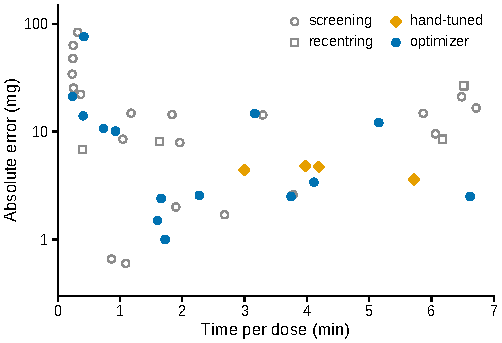
\includegraphics[max width=\linewidth]{fig1_time_vs_error}
  \figcaption{fig1_time_vs_error}
  \label{fig:time-vs-error}
\end{figure}

\begin{figure*}[ht]
  \centering
  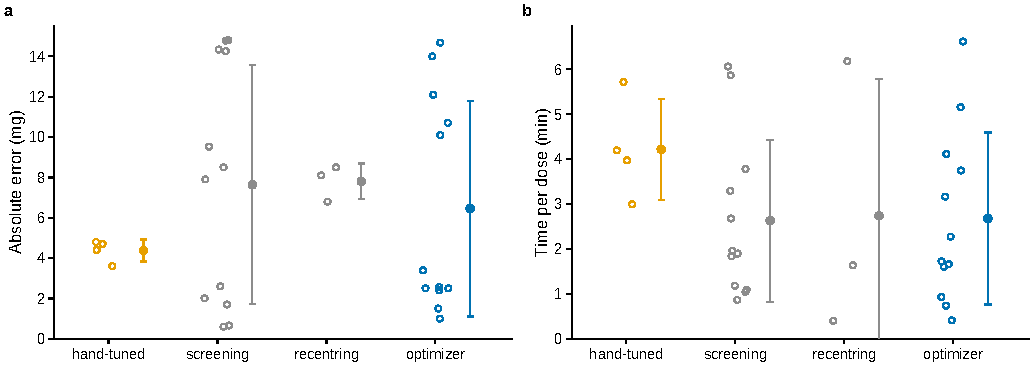
\includegraphics[max width=\linewidth]{fig2_group_spread}
  \figcaption{fig2_group_spread}
  \label{fig:group-spread}
\end{figure*}

Figure~\ref{fig:time-vs-error} shows \fillme{the finding}, and
Fig.~\ref{fig:group-spread} \fillme{the comparison}.

\section{Discussion}\label{sec:discussion}
\fillme{What the results mean, how they compare with prior work, and the limits:
what was not tested, the size of n, and what would change the conclusion.}

\section{Conclusions}\label{sec:conclusions}
\fillme{Three to five sentences: what was done, the main number, what it enables.}


\section*{Author contributions}
% Written by scripts/credit.py from credit.csv: edit the CSV, then make credit.
\textbf{First Author}: \fillme{roles}. \textbf{Second Author}: \fillme{roles}. \textbf{Sterling G. Baird}: \fillme{roles}.


\section*{Conflicts of interest}
% RSC's wording when there are none: "There are no conflicts to declare."
% Conflict of interest: confirm with every author (the sign-off checklist asks)
% before deleting the marker. An author with a relevant patent, company,
% consultancy or equity names it here instead.
\fillme{Every author has confirmed:} The authors declare no competing interests.


\section*{Data availability}
% Data and code availability: one paragraph for every publisher; the main-*.tex
% gives it the heading its journal uses. Fill, do not invent: each \fillme
% names something that must exist before submission.
% Zenodo reserves a DOI before a record is published (in the upload form,
% "Do you already have a DOI?" -> No -> "Get a DOI now!"), so the manuscript
% can carry the real DOI at submission. A GitHub release archived through
% Zenodo's GitHub integration also works.
The data behind every figure (snapshots, each with a README stating units,
sample size and provenance), the scripts that draw the figures, and
\fillme{the analysis, control or design files} are archived on Zenodo at
\fillme{https://doi.org/10.5281/zenodo.NNNNNNN} under \fillme{licence:
CC BY 4.0 for data, MIT for code}. Development continues at
\fillme{https://github.com/vertical-cloud-lab/REPOSITORY}.
\fillme{Anything not shared, and why; or delete this sentence.}


\section*{Acknowledgements}
\fillme{People who helped but are not authors, with their permission to be
named; facilities and shared instruments.}

% Funding: one line per award, with the funder named as in the Crossref Funder
% Registry (https://www.crossref.org/services/funder-registry/) and the award
% number exactly as on the award letter. Copy it from the award, never from
% memory or from another paper; ask the PI for the list at G3.
This work was supported by \fillme{funder} under award \fillme{number}.
\fillme{One sentence per further award, including any student fellowship or
mentored-research award, worded as its recipient confirms.}

\fillme{Generative AI: the tool and version, as in the statement in Methods.}

\balance

\bibliography{references}
\bibliographystyle{rsc}
\end{document}
